\documentclass[10pt]{beamer}
\usetheme{Madrid}
\usepackage[utf8]{inputenc}
\usepackage[russian]{babel}
\usepackage[OT1]{fontenc}
\usepackage{amsmath}
\usepackage{amsfonts}
\usepackage{amssymb}
\usepackage{graphicx}
\usepackage{scrextend}
\author{Мальковский Н.~В.}
\title[Метод Ньютона]{Метод Ньютона}
%\setbeamercovered{transparent} 
\setbeamertemplate{navigation symbols}{} 
\graphicspath{{image/}}
%\logo{} 
\institute[СПбАУ]{Санкт-Петербургский Академический  Университет}
\date{} 
\usecolortheme{beaver}
%\subject{} 

\DeclareMathOperator{\argmin}{argmin}
\DeclareMathOperator{\interior}{Int}
\DeclareMathOperator{\lin}{Span}
\DeclareMathOperator{\llin}{Lin}
\DeclareMathOperator{\diag}{diag}



%\setbeamertemplate{theorems}[numbered]

\newcounter{thm}
\newcounter{lm}
\newcounter{def}


\newtheorem{theorem_ru}[thm]{Теорема}
\newtheorem{lemma_ru}[lm]{Лемма}
\newtheorem{corollary_ru}{Следствие}[]
\newtheorem{definition_ru}{Определение}[def]

\newcommand{\Ima}{\text{Im}}
\newcounter{remarknumber}[framenumber]
\newcommand{\remark}{\stepcounter{remarknumber}\textit{Замечание}~\arabic{remarknumber}}


\begin{document}

\begin{frame}
\titlepage
\centering
\includegraphics[width=.23\textwidth]{logo.png}
\end{frame}

\begin{frame}{Метод Ньютона и градиентный спуск}
Градиентный спуск:
$$
x_{k+1}=x_k-\alpha_k\nabla f(x_k).
$$
\pause
Основная формальная модификация метода Ньютона:
$$
\alpha_k\rightarrow \alpha(x)\in \mathbb{R}^{n\times n}
$$
\pause
Общая идея: на каждом шаге минимизируем квадратичное приближение $f$:
$$
x_{k+1}=\argmin_x (f(x_k)+\nabla f(x_k)^T(x-x_k)+\frac{1}{2}(x-x_k)\nabla^2f(x_k)(x-x_k))
$$
\pause
Условия оптимальности первого рода дают уравнение на $x_{k+1}$:
$$
\nabla f(x_k)+\nabla^2f(x_k)(x-x_k)=0
$$
Таким образом
\begin{equation}\label{newton_method}
x_{k+1}=x_k-[\nabla^2 f(x_k)]^{-1}\nabla f(x_k)
\end{equation}
\end{frame}

\begin{frame}{За и против}
Плюсы:
\pause
\begin{itemize}
\item Сходится гораздо быстрее.
\end{itemize}
\pause
Минусы:
\begin{itemize}[<+->]
\item Нужна возможность измерить гессиан $\nabla^2 f(x_k)$
\item Больше вычислений на итерацию: необходимо либо обращать гессиан, либо решать систему
$$
\nabla^2f(x_k)(x-x_k)=-\nabla f(x_k)
$$
\end{itemize}
\end{frame}

\begin{frame}{Метод Ньютона для уравнений}
Рассмотрим систему уравнений
$$
f(x)=0_n,
$$
где $f:\mathbb{R}^n\rightarrow\mathbb{R}^n$, $f$ дифференцируема.\\
\vspace{1em}
\pause
Аналогично задаче минимизации, метод Ньютона для решение системы уравнений заключается в замене исходной системы на её линейное приближение и последовательное итерирование. Решение линейной системы:
$$
x_{k+1}: f(x_k)+\nabla f(x_k)(x_{k+1}-x_k)=0~~\Rightarrow
$$
что дает
\begin{equation}\label{newton_method_root}
x_{k+1}=x_k-\nabla f(x_k)^{-1}f(x_k)
\end{equation}
\end{frame}

\begin{frame}{Метод Ньютона в одномерном случае}
\only<1-1>{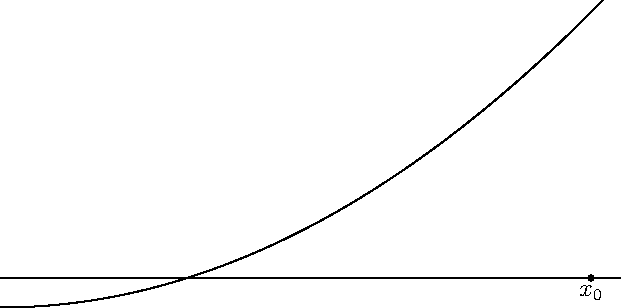
\includegraphics[width=\textwidth]{newton/newton_sqrt0}}%
\only<2-2>{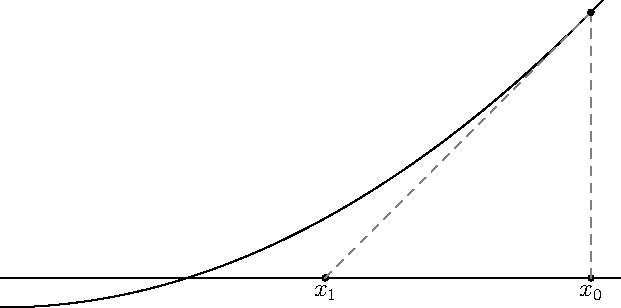
\includegraphics[width=\textwidth]{newton/newton_sqrt1}}%
\only<3-3>{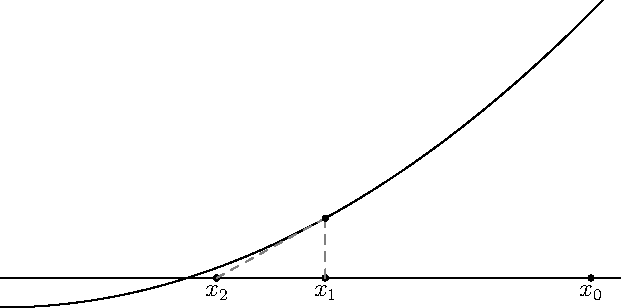
\includegraphics[width=\textwidth]{newton/newton_sqrt2}}%
\only<4-4>{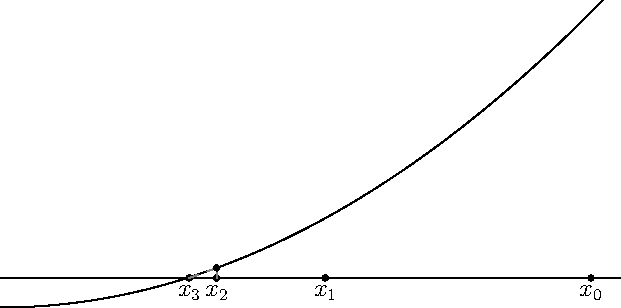
\includegraphics[width=\textwidth]{newton/newton_sqrt3}}%
\end{frame}

\begin{frame}{Пример: вычисление обратной функции}
Предположим, что мы умеем вычислять $f(x)$ и $\nabla f(x)$, хотим научиться вычислять $f^{-1}(x)$.\\
\vspace{1em}
\pause
Пусть $f^{-1}(y^*)=x^*$, тогда $f(x^*)=y^*$, отсюда вычисление $f^{-1}(y^*)$ равносильно решению системы
$$
f(x)-y^*=0.
$$
\pause
Используя метод Ньютона получаем алгоритм
$$
x_{k+1}=x_k-[\nabla f(x)]^{-1}(f(x_k)-y^*)
$$
\end{frame}

\begin{frame}{Пример: вычисления вещественного корня}
Пусть $f(x)=x^2$, $f^{-1}(x)=\sqrt{x}$, тогда рассмотренная схема имеет вид
$$
x_{k+1}=x_k-\frac{x_k^2-y^*}{2x_k}=\frac{1}{2}\left(x_k+\frac{y^*}{x_k}\right)
$$
\pause
Функция $g(x)=\frac{1}{2}\left(x-\frac{y^*}{x}\right)$ имеет две неподвижные точки $\pm\sqrt{y^*}$, а значит последовательность $x_{k+1}=g(x_k)$ сходится либо к одной из них\\
\vspace{1em}
Очевидным образом, если $x>0$, то $g(x)>0$ и наоборот. Следовательно, если $x_0>0$, то последовательность сходится к $\sqrt{y^*}$, а если $x_0<0$, то последовательность сходится к $-\sqrt{y^*}$.

\end{frame}

\begin{frame}{Анализ сходимости}
Рассмотрим близкий к \eqref{newton_method_root} метод: \begin{equation}\label{aux_newton}
x_{k+1}=x_k-[\nabla f(x^*)]^{-1}f(x_k)
\end{equation}
\pause
Этот метод представляет только теоретическую ценность, так как предполагает возможность вычисления $\nabla f(x^*)$, что практически не осуществимо без знания $x^*$.\\
\pause
\vspace{1em}
Пусть $g(x)=x-[\nabla f(x^*)]^{-1}f(x)$, тогда \eqref{aux_newton} имеет вид
$$
x_{k+1}=g(x_k)
$$
и при этом
$$
\nabla g(x)=I-[\nabla f(x^*)]^{-1}\nabla f(x).
$$
\pause
Таким образом, $g(x^*)=0$ и $\nabla g$ удовлетворяет условию Липшица, если $\nabla f$ удовлетворяет. 

\end{frame}

\begin{frame}{Анализ сходимости}
Используя теорему о квадратичной сходимости для рекуррентных процессов получаем
\begin{theorem_ru}
Если $f$ дифференцируема на $S=\{x~|~||x-x^*||\leq ||x_0-x^*||\}$, $\det \nabla f(x^*)\neq 0$, $\nabla f$ удовлетворяет условию Липшица с константой $L$ на $S$ и $q=\frac{1+||[\nabla f(x^*)]^{-1}||L}{2}||x_0-x^*||<1$, то для последовательности \eqref{aux_newton} выполняется
$$
||x_k-x^*||\leq \frac{2}{||\nabla f(x^*)||L}q^{2^k}
$$
\end{theorem_ru}
\pause
\textbf{Док-во} Применяем теорему о квадратичной сходимости для $g(x)=x-[\nabla f(x^*)]^{-1}f(x)$ и учитываем, что
\begin{align*}
||\nabla g(x)-\nabla g(y)||&=||[\nabla f(x^*)]^{-1}(\nabla f(x)-\nabla f(y))+(x-y)||\\
&\leq (1+||[\nabla f(x^*)]^{-1}||L)||x-y||~~\blacksquare
\end{align*}
\end{frame}

\begin{frame}{Анализ сходимости}
Возвращаемся к \eqref{newton_method}.
\begin{theorem_ru}[О скорости сходимости метода Ньютона для задач оптимизации]
Пусть $f:\mathbb{R}^n\rightarrow \mathbb{R}$ дважды дифференцируема на $S=\left\{||x-x^*||\leq\frac{m}{\gamma M}\right\}$ 
при некотором $\gamma\geq 3/2$, $x^*$ -- точка минимума $f$ на $S$ и $mI\preceq\nabla^2 f(x^*)$ при $m>0$, для $\nabla^2 f$ на $S$ выполняется условие Липшица с константой $M$, $x_0\in S$, 
тогда для последовательности \eqref{newton_method} выполняется
$$
||x_{k+1}-x^*||\leq \frac{M||x_k-x^*||^2}{2(m-M||x_k-x^*||)}
$$
\end{theorem_ru}
\pause
\textbf{Док-во.} Обозначим $G_k= \int_0^1[\nabla^2 f(x_k)-\nabla^2 f(x^*+t(x_k-x^*))]dt$, тогда
\begin{align*}
x_{k+1}-x^*&=x_k-x^*-[\nabla^2 f(x_k)]^{-1}\nabla f(x_k)\\
&=x_k-x^*-[\nabla^2 f(x_k))]^{-1}\int_0^1\nabla^2 f(x^*+t(x_k-x^*))(x_k-x^*)dt \\
&=[\nabla^2 f(x_k)]^{-1}G_k(x-x^*).
\end{align*}
\end{frame}

\begin{frame}{Анализ сходимости}
Далее
\begin{align*}
||G_k||&=\left\|\int_0^1[\nabla^2 f(x_k)-\nabla^2 f(x^*+t(x_k-x^*))]dt\right\|\\
&\leq \int_0^1||[\nabla^2 f(x_k)-\nabla^2 f(x^*+t(x_k-x^*))]||dt \\
&\leq \int_0^1M(1-t)||x_k-x^*||dt\\
&=\frac{M||x_k-x^*||}{2}
\end{align*}
\pause
Вновь используя условие Липшица для $\nabla^2 f$ получаем, что 
$$
-M||x_k-x^*||I\preceq\nabla^2 f(x_k)-\nabla^2 f(x^*)\preceq M||x_k-x^*||I,
$$
\pause что дает
$$
(m-M||x_k-x^*||)I\preceq \nabla^2 f(x^*)-M||x_k-x^*||I\preceq \nabla^2 f(x_k)
$$
\pause
Если $x_k\in S$, то $M||x_k-x^*||-m>0$, а $\nabla^2 f(x_k)$ обратима и при этом
$$
||[\nabla^2 f(x_k)]^{-1}||\leq (m-M||x_k-x^*||)^{-1}
$$ 

\end{frame}

\begin{frame}{Анализ сходимости}
Итог:
$$
||x_{k+1}-x^*||\leq \frac{M||x_k-x^*||^2}{2(m-M||x_k-x^*||)}
$$
что дает оценку скорости сходимости.\\
\vspace{1em}
\pause
Осталось показать, что $||x_{k+1}-x^*||\leq ||x_k-x^*||$, чтобы гарантировать $x_k\in S$:
\begin{align*}
\frac{M||x_k-x^*||^2}{2(m-M||x_k-x^*||)}&\leq ||x_k-x^*||~~\Leftrightarrow\\
M||x_k-x^*||^2&\leq 2(m-M||x_k-x^*||)||x_k-x^*||~~\Leftrightarrow\\
3M||x_k-x^*||^2&\leq 2m||x_k-x^*||.
\end{align*}
\pause
Таким образом, если $\gamma\geq 3/2$, то $||x_{k+1}-x^*||\leq ||x_k-x^*||$, $x_0\in S$ и $x_k\in S$.~~$\blacksquare$
\end{frame}

\begin{frame}{Ссылки на литературу}
\href{http://premolab.ru/pub_files/pub5/MnexoB89z7.pdf}{\textit{Нестеров Ю. Е.} Методы выпуклой оптимизации}
 // параграф 1.2.4\\
 \vspace{1em}

\href{https://web.stanford.edu/class/ee364a/lectures/unconstrained.pdf}{\textit{Vandenberghe L.} Unconstrained optimization (slides)}
\end{frame}


\end{document}